\section{KHẢO SÁT SỰ BIẾN THIÊN VÀ VẼ ĐỒ THỊ HÀM SỐ}
%\subsection{LÝ THUYẾT CẦN NHỚ}
\subsubsection{Hàm số bậc ba $\mathbf{y=ax^3+bx^2+cx+d}$}
	\begin{minipage}[b]{12cm}
		\begin{enumerate}[\iconCH]
			\item \indamm{TH1.} $y'=0$ có hai nghiệm phân biệt $x_1$ và $x_2$. Khi đó, hàm số có hai điểm cực trị $x=x_1$ và $x=x_2$.\\
			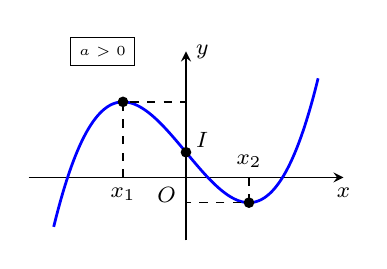
\begin{tikzpicture}[smooth,samples=300,line width=0.6pt,scale=0.8,>=stealth,font=\footnotesize]
				\draw[->] (-2.5,0)--(2.5,0) node[below]{$x$};
				\draw[->] (0,-1)--(0,2) node[right]{$y$};
				\draw (0,0) node[below left]{$O$};
				\draw[blue,line width=1pt,domain=-2.1:2.1] plot(\x,{0.4*((\x)^3-3*(\x)+1)});
				\draw[fill=black] (0,0.4) circle(2pt) (-1,1.2) circle(2pt) (1,-0.4) circle(2pt);
				\draw[dashed] (1,0)node[above]{\footnotesize$x_2$}--(1,-0.4)--(0,-0.4) (-1,0)node[below]{\footnotesize$x_1$}--(-1,1.2)--(0,1.2);
				\node[right] at (0,0.6) {\footnotesize $I$};
				\node[right] at (-2,2) {\tiny\fbox{$a>0$}};
			\end{tikzpicture}
			\hspace{0.3cm}
			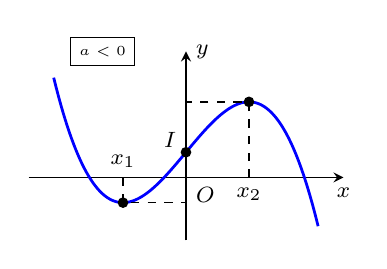
\begin{tikzpicture}[smooth,samples=300,line width=0.6pt,scale=0.8,>=stealth,font=\footnotesize]
				\draw[->] (-2.5,0)--(2.5,0) node[below]{$x$};
				\draw[->] (0,-1)--(0,2) node[right]{$y$};
				\draw (0,0) node[below right]{$O$};
				\draw[blue,line width=1pt,domain=-2.1:2.1] plot(\x,{0.4*(-(\x)^3+3*(\x)+1)});
				\draw[fill=black] (0,0.4) circle(2pt) (1,1.2) circle(2pt) (-1,-0.4) circle(2pt);
				\draw[dashed] (-1,0)node[above]{\footnotesize$x_1$}--(-1,-0.4)--(0,-0.4) (1,0)node[below]{\footnotesize$x_2$}--(1,1.2)--(0,1.2);
				\node[left] at (0,0.6) {\footnotesize$I$};
				\node[right] at (-2,2) {\tiny\fbox{$a<0$}};
			\end{tikzpicture}
			\item \indamm{TH2.} $y'=0$ có nghiệm kép $x_0$. Khi đó, hàm số không có cực trị.\\
			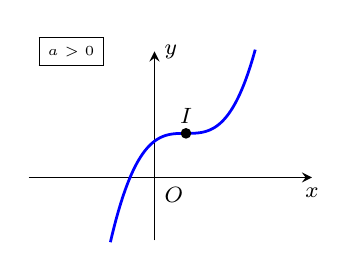
\begin{tikzpicture}[smooth,samples=300,line width=0.6pt,scale=0.8,>=stealth,font=\footnotesize]
				\draw[->] (-2,0)--(2.5,0) node[below]{$x$};
				\draw[->] (0,-1)--(0,2) node[right]{$y$};
				\draw (0,0) node[below right]{$O$};
				\draw[blue,line width=1pt,domain=-0.7:1.6] plot(\x,{(\x-0.5)^3+0.7});
				\draw[fill=black] (0.5,0.7) circle(2pt);
				\node[above] at (0.5,0.7) {\footnotesize$I$};
				\node[right] at (-2,2) {\tiny\fbox{$a>0$}};
			\end{tikzpicture}
			\hspace{0.5cm}
			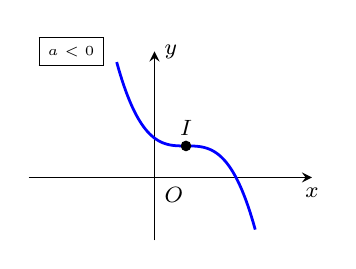
\begin{tikzpicture}[smooth,samples=300,line width=0.6pt,scale=0.8,>=stealth,font=\footnotesize]
				\draw[->] (-2,0)--(2.5,0) node[below]{$x$};
				\draw[->] (0,-1)--(0,2) node[right]{$y$};
				\draw (0,0) node[below right]{$O$};
				\draw[blue,line width=1pt,domain=-0.6:1.6] plot(\x,{-((\x-0.5)^3-0.5)});
				\draw[fill=black] (0.5,0.5) circle(2pt);
				\node[above] at (0.5,0.5) {\footnotesize$I$};
				\node[right] at (-2,2) {\tiny\fbox{$a<0$}};
			\end{tikzpicture}
			\item \indamm{TH3.} $y'=0$ vô nghiệm. Khi đó, hàm số không có cực trị.\\
			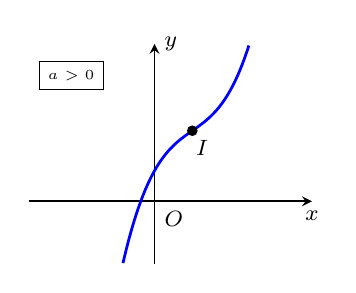
\begin{tikzpicture}[smooth,samples=300,line width=0.6pt,scale=0.8,>=stealth,font=\footnotesize]
				\draw[->] (-2,0)--(2.5,0) node[below]{$x$};
				\draw[->] (0,-1)--(0,2.5) node[right]{$y$};
				\draw (0,0) node[below right]{$O$};
				\draw[blue,line width=1pt,domain=-0.5:1.5] plot(\x,{((\x-0.6)^3+0.7*(\x)+0.7)});
				\draw[fill=black] (0.6,1.12) circle(2pt);
				\node[below right] at (0.5,1.12) {\footnotesize$I$};
				\node[right] at (-2,2) {\tiny\fbox{$a>0$}};
			\end{tikzpicture}
			\hspace{0.5cm}
			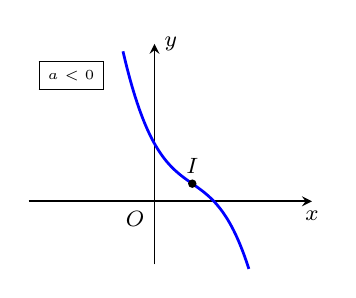
\begin{tikzpicture}[smooth,samples=300,line width=0.6pt,scale=0.8,>=stealth,font=\footnotesize]
				\draw[->] (-2,0)--(2.5,0) node[below]{$x$};
				\draw[->] (0,-1)--(0,2.5) node[right]{$y$};
				\draw (0,0) node[below left]{$O$};
				\draw[blue,line width=1pt,domain=-0.5:1.5] plot(\x,{-(\x-0.6)^3-0.7*(\x)+0.7)});
				\draw[fill=black] (0.6,0.28) circle(1.5pt);
				\node[right] at (-2,2) {\tiny\fbox{$a<0$}};
				\node[above] at (0.6,0.28) {\footnotesize$I$};
			\end{tikzpicture}
		\end{enumerate}
		\vspace{0.4cm}
	\end{minipage}\hspace{0.32cm}
	\begin{minipage}[b]{6.8cm}
		\begin{khung4}{GHI NHỚ}
			\ding{172} Hàm số không có điểm cực trị
			$$b^2-3ac\le 0 \text{ hoặc } \heva{&a=0 \\&b=0.}$$
			\ding{173} Hàm số có hai điểm cực trị
			$$\heva{&a \ne 0\\&b^2-3ac >0.}$$
			\ding{174} Liên hệ tổng tích hai nghiệm
			$$\heva{&x_1+x_2=-\dfrac{2b}{3a}\\&x_1x_2=\dfrac{c}{3a}}$$
			\ding{175}  Hoành độ tâm đối xứng là nghiệm phương trình $y''=0 \Leftrightarrow x=-\dfrac{b}{3a}$.\\
			\ding{176} Tiếp tuyến tại tâm đối xứng sẽ có hệ số góc nhỏ nhất nếu $a>0$ và lớn nhất nếu $a<0$.
		\end{khung4}
\vspace{1cm}
	\end{minipage}

\subsubsection{Hàm số $\mathbf{y = \dfrac{{ax + b}}{{cx + d}}\left( {c \ne 0,ad - bc \ne 0} \right)}$}
\begin{minipage}[b]{12cm}
	\begin{enumerate}[\iconCH]
		\item Tập xác định $D=\mathbb{R}\backslash \left\{-\dfrac{d}{c}\right\}$; Đạo hàm $y'=\dfrac{ad-cb}{(cx+d)^2}$.
		\item Đồ thị nhận giao điểm của hai đường tiệm cận làm tâm đối xứng.
		\item Hình dạng đồ thị:\\
		\begin{tikzpicture}[smooth,samples=300,line width=0.6pt,>=stealth, scale=0.45]
			\draw[->] (-5,0)--(3.5,0) node[below]{$x$};
			\draw[->] (0,-1.6)--(0,5.7) node[right]{$y$};
			\draw (0,0) node[below right]{$O$};
			\node at (-3,5.3) {\tiny\fbox{$y'>0$}};
			\clip (-5,-1.5) rectangle (3,5.5);
			\draw[dashed] (-1,-2)--(-1,5.5) (-5,2)--(3,2);
			\draw[blue,line width=1pt,domain=-5:-1.1] plot(\x,{(2*(\x)+1)/((\x)+1)});
			\draw[blue,line width=1pt,domain=-0.9:3] plot(\x,{(2*(\x)+1)/((\x)+1)});
			\draw[fill=black] (-1,2) circle(1.5pt) circle(1.5pt) (-1,0) circle(1pt) (0,2) circle(1pt);
			\node[left] at (-1,1.5) {\footnotesize $I$};
			\node[below left] at (-1,0) {\tiny $-\dfrac{d}{c}$};
			\node[above right] at (0,2) {\tiny $\dfrac{a}{c}$};
		\end{tikzpicture}
		\hspace{0.5cm}
		\begin{tikzpicture}[smooth,samples=300,line width=0.6pt,>=stealth, scale=0.45]
			\draw[->] (-3,0)--(5.5,0) node[below]{$x$};
			\draw[->] (0,-1.6)--(0,5.7) node[left]{$y$};
			\draw (0,0) node[below left]{$O$};
			\node at (3,5.3) {\tiny \fbox{$y'<0$}};
			\clip (-3,-1.5) rectangle (5,5.5);
			\draw[dashed] (1,-2)--(1,5.5) (-3,2)--(5,2);
			\draw[blue,line width=1pt,domain=-3:0.9] plot(\x,{(2*(\x)-1)/((\x)-1)});
			\draw[blue,line width=1pt,domain=1.1:5] plot(\x,{(2*(\x)-1)/((\x)-1)});
			\draw[fill=black] (1,2) circle(1.5pt) (1,0) circle(1pt) (0,2) circle(1pt);
			\node[right] at (1,1.5) {\footnotesize $I$};
			\node[below right] at (1,0) {\tiny $-\dfrac{d}{c}$};
			\node[above left] at (0,2) {\tiny $\dfrac{a}{c}$};
		\end{tikzpicture}
	\end{enumerate}
\end{minipage}\hspace{0.5cm}
\begin{minipage}[b]{6.8cm}
	\begin{khung4}{GHI NHỚ}
		\ding{172} Tiệm cận đứng $x=-\dfrac{d}{c}$.\\
		\ding{173} Tiệm cận ngang $y=\dfrac{a}{c}$.\\
		\ding{174} Giao với $Ox$: $y=0 \Rightarrow x=-\dfrac{b}{a}$.\\
		\ding{175} Giao với $Oy$: $x=0 \Rightarrow y=\dfrac{b}{d}$.\\
	\end{khung4}
	\vspace{1cm}
\end{minipage}
\subsubsection{Hàm số $\mathbf{y = \dfrac{{a{x^2} + bx + c}}{{mx + n}}\left( {a \ne 0,m \ne 0} \right)}$ (đa thức tử không chia hết cho đa thức mẫu)}
\begin{enumerate}[\iconCH]
	\item Tập xác định $D=\mathbb{R}\backslash \left\{-\dfrac{n}{m}\right\}$; Đạo hàm $y'=\dfrac{am\cdot x^2+2an\cdot x + b.n - m.c}{(mx+n)^2}$.
	\item Hàm số $2$ điểm cực trị khi $y'=0$ có $2$ nghiệm phân biệt; Hàm số không có cực trị khi $y'=0$ vô nghiệm.
	\item Đồ thị nhận giao điểm của tiệm cận đứng và tiệm cận xiên làm tâm đối xứng.
	\item Hình dạng đồ thị:\\
	\begin{tikzpicture}[line cap=butt,line join=miter,>=stealth,scale=0.4,font=\footnotesize]
		\tikzset{declare function={xmin=-5.5;xmax=3.5;ymin=-4.6;ymax=4.6;},
			smooth,samples=450}
		\draw[->] (xmin,-0.5)--(xmax,-0.5) node[above]{$ x $};
		\draw[->] (0,ymin)--(0,ymax) node[right]{$ y $};
		\fill (0,-0.5) node[above right]{$ O $};
		\path (current bounding box.south) node[below, black]{\tiny\fbox{$a>0$, $y'=0$ có $2$ nghiệm phân biệt}};
		\clip (xmin,ymin) rectangle (xmax,ymax);
		\def\f(#1){((#1)^2+2*(#1)+2)/((#1)+1)} % Hàm số
		\def\q(#1){((#1)+1)} % Tiệm cận xiên	
		\draw[blue,thick,samples=250] plot[domain=xmin:-1.1] (\x,{\f(\x)});	
		\draw[blue,thick,samples=250] plot[domain=-0.9:xmax] (\x,{\f(\x)});
		%--------- Tiệm cận
		\draw[dashed] plot [domain=xmin:xmax] (\x,{\q(\x)}) ;
		\draw[dashed] (-1,ymin)--(-1,ymax);
	\end{tikzpicture}	
	\hspace{.25cm}
	\begin{tikzpicture}[line cap=butt,line join=miter,>=stealth,scale=0.4,font=\footnotesize]
		\tikzset{declare function={xmin=-5.5;xmax=3.5;ymin=-4.6;ymax=4.6;},
			smooth,samples=450}
		\draw[->] (xmin,-0.5)--(xmax,-0.5) node[above]{$ x $};
		\draw[->] (0,ymin)--(0,ymax) node[right]{$ y $};
		\fill (0,-0.5) node[above right]{$ O $};
		\path (current bounding box.south) node[below, black]{\tiny\fbox{$a<0$, $y'=0$ có $2$ nghiệm phân biệt}};
		\clip (xmin,ymin) rectangle (xmax,ymax);
		\def\f(#1){(-(#1)^2-2*(#1)-2)/((#1)+1)} % Hàm số
		\def\q(#1){(-(#1)-1)} % Tiệm cận xiên	
		\draw[blue,thick,samples=250] plot[domain=xmin:-1.1] (\x,{\f(\x)});	
		\draw[blue,thick,samples=250] plot[domain=-0.9:xmax] (\x,{\f(\x)});
		%--------- Tiệm cận
		\draw[dashed] plot [domain=xmin:xmax] (\x,{\q(\x)}) ;
		\draw[dashed] (-1,ymin)--(-1,ymax);
	\end{tikzpicture}	
	\hspace{.25cm}
	\begin{tikzpicture}[line cap=butt,line join=miter,>=stealth,scale=0.4,font=\footnotesize]
		\tikzset{declare function={xmin=-5.5;xmax=3.5;ymin=-4.6;ymax=4.6;},
			smooth,samples=450}
		\draw[->] (xmin,-0.5)--(xmax,-0.5) node[above]{$ x $};
		\draw[->] (0,ymin)--(0,ymax) node[right]{$ y $};
		\fill (0,-0.5) node[above right]{$ O $};
		\path (current bounding box.south) node[below, black]{\tiny\fbox{$a>0$, $y'=0$ vô nghiệm}};
		\clip (xmin,ymin) rectangle (xmax,ymax);
		\def\f(#1){((#1)^2+2*(#1))/((#1)+1)} % Hàm số
		\def\q(#1){((#1)+1)} % Tiệm cận xiên	
		\draw[blue,thick,samples=250] plot[domain=xmin:-1.1] (\x,{\f(\x)});	
		\draw[blue,thick,samples=250] plot[domain=-0.9:xmax] (\x,{\f(\x)});
		%--------- Tiệm cận
		\draw[dashed] plot [domain=xmin:xmax] (\x,{\q(\x)}) ;
		\draw[dashed] (-1,ymin)--(-1,ymax);
	\end{tikzpicture}	
	\hspace{.25cm}
	\begin{tikzpicture}[line cap=butt,line join=miter,>=stealth,scale=0.4,font=\footnotesize]
		\tikzset{declare function={xmin=-5.5;xmax=3.5;ymin=-4.6;ymax=4.6;},
			smooth,samples=450}
		\draw[->] (xmin,-0.5)--(xmax,-0.5) node[above]{$ x $};
		\draw[->] (0,ymin)--(0,ymax) node[right]{$ y $};
		\fill (0,-0.5) node[above right]{$ O $};
		\path (current bounding box.south) node[below, black]{\tiny\fbox{$a<0$, $y'=0$ vô nghiệm}};
		\clip (xmin,ymin) rectangle (xmax,ymax);
		\def\f(#1){(-(#1)^2-2*(#1))/((#1)+1)} % Hàm số
		\def\q(#1){(-(#1)-1)} % Tiệm cận xiên	
		\draw[blue,thick,samples=250] plot[domain=xmin:-1.1] (\x,{\f(\x)});	
		\draw[blue,thick,samples=250] plot[domain=-0.9:xmax] (\x,{\f(\x)});
		%--------- Tiệm cận
		\draw[dashed] plot [domain=xmin:xmax] (\x,{\q(\x)}) ;
		\draw[dashed] (-1,ymin)--(-1,ymax);
	\end{tikzpicture}
\end{enumerate}
